% begin module arctan-def
\begin{frame}
\begin{columns}[c]
\column{.5\textwidth}
\psset{xunit=0.6cm, yunit=0.6cm}
\begin{pspicture}(-3.9, -3.8)(5.2,3.8) 
\psframe*[linecolor=white](-3.9,3.8)(5.2,3.8) 
\tiny 
\psaxesStandard{-3.85}{-3.7}{5.2}{3.7}
%Function formula: \frac{\sin{}x}{\cos{}x} 

\uncover<1>{
\psplot[linecolor=\psColorGraph, plotpoints=1000]{-3.8}{-1.841592654}{x 57.29578 mul tan }
}
\uncover<1-2>{
\psplot[linecolor=\psColorGraph, plotpoints=1000]{-1.3}{1.3}{x 57.29578 mul tan }
}
\uncover<3->{
\psplot[linecolor=gray, plotpoints=1000]{-1.3}{1.3}{x 57.29578 mul tan }
}
\uncover<1>{
\psplot[linecolor=\psColorGraph, plotpoints=1000]{1.841592654}{4.441592654}{x 57.29578 mul tan }
}
\uncover<3->{
\psplot[linecolor=\psColorGraph, plotpoints=1000]{-3.602102448}{3.602102448}{x ATAN }
}
\uncover<1-2>{
\psline[linestyle=dashed](1.570796327, -3.7)(1.570796327, 3.7)
\psline[linestyle=dashed](-1.570796327, -3.7)(-1.570796327, 3.7)
}
\uncover<3->{
%\psline[linecolor=gray!20, linestyle=dashed](1.570796327, -3.7)(1.570796327, 3.7)
%\psline[linecolor=gray!20, linestyle=dashed](-1.570796327, -3.7)(-1.570796327, 3.7)
\psline[linestyle=dashed](-3.7, 1.570796327)(5, 1.570796327)
\psline[linestyle=dashed](-3.7, -1.570796327)(5, -1.570796327)
}
\uncover<1>{
\psline[linestyle=dashed](4.71238898, -3.7)(4.71238898, 3.7)
}
\uncover<3->{
\psline(1.570796327, -0.1)(1.570796327, 0.1)
\psline(-1.570796327, -0.1)(-1.570796327, 0.1)
}
\rput[tr](1.5,-0.1){$\frac{\pi}{2}$}
\rput[tr](-1.7,-0.1){$-\frac{\pi}{2}$}
\uncover<1>{
\psXTickWithLabel{3.141592654}{$\pi$}
\psXTickWithLabel{-3.141592654}{$-\pi$}
}
\uncover<1>{\rput[tr](4.65,-0.1){$\frac{3\pi}{2}$}
}
\psYTickWithLabel{1}{$1$}
\psYTickWithLabel{-1}{$-1$}
\rput[l](1.6, 2.1){ $\begin{array}{l} y=\tan x\uncover<2->{,}\\ \uncover<2->{-\frac{\pi}{2}\leq x\leq\frac{\pi}{2} }\end{array}$
}
\end{pspicture} 

%\ \only<handout:0| -1>{%
%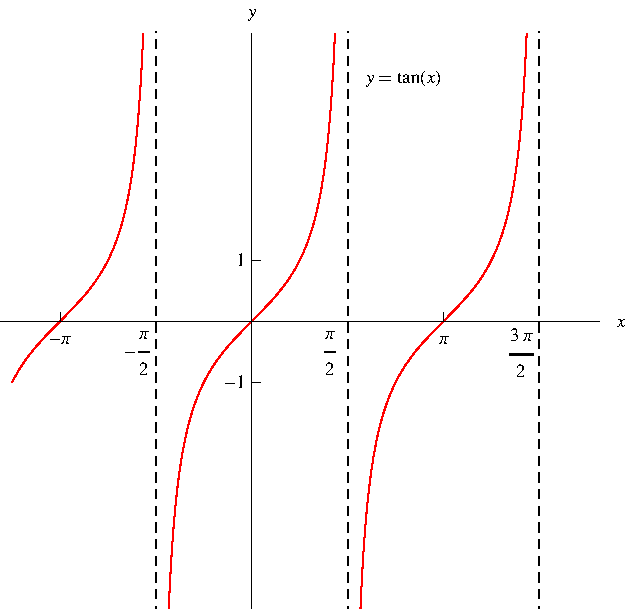
\includegraphics[width=5cm]{inverse-trig/pictures/07-06-arctana.pdf}%
%}%
%\only<handout:1| 2>{%
%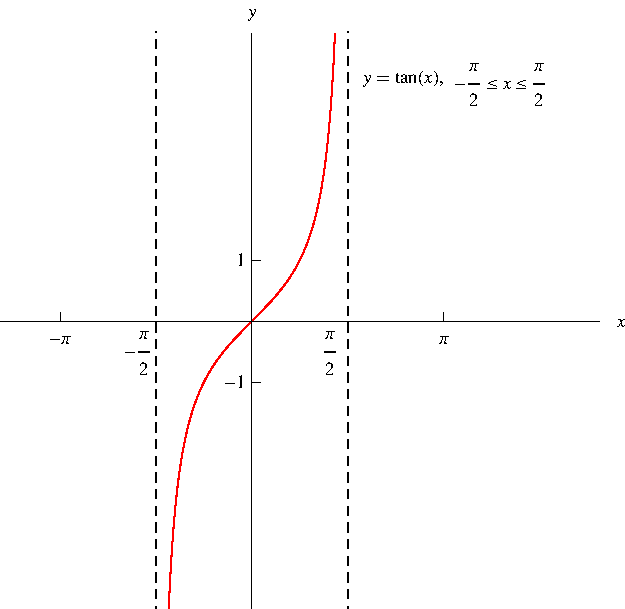
\includegraphics[width=5cm]{inverse-trig/pictures/07-06-arctanb.pdf}%
%}%
%\only<handout:2| 3->{%
%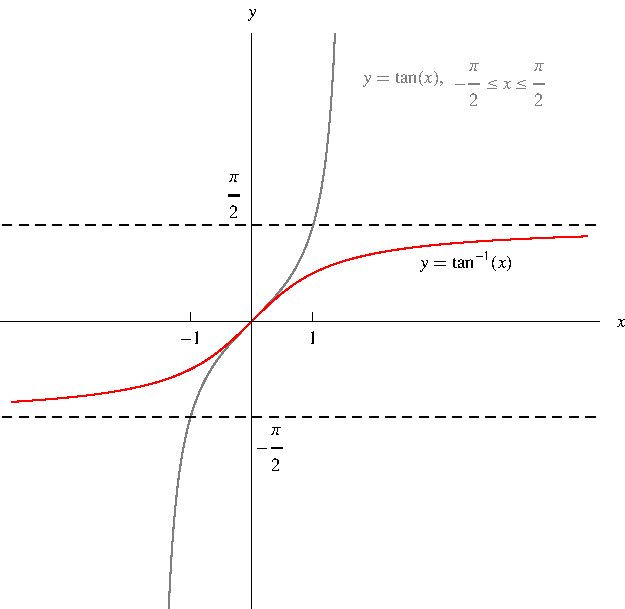
\includegraphics[width=5cm]{inverse-trig/pictures/07-06-arctanc.pdf}%
%}%
\column{.5\textwidth}
\begin{itemize}
\item<1->  $\tan x$ isn't one-to-one.
\item<2->  Restrict the domain to $(-\frac{\pi}2, \frac{\pi}2)$.
\item<3->  The inverse is called $\Arctan$ or $\arctan$.
\item<4->  $\Arctan x = y \Leftrightarrow \tan y = x$ and $-\frac{\pi}2 < y < \frac{\pi}2$.
\item<5->  \alert<handout:0| 5-6>{Domain of $\Arctan$: \uncover<6-| handout:0>{$(-\infty,\infty)$.}}
\item<5->  \alert<handout:0| 7-8>{Range of $\Arctan$: \uncover<8-| handout:0>{$(-\frac{\pi}2, \frac{\pi}2 )$.}}
\item<9->  \alert<handout:0| 9-10>{$\displaystyle \lim_{x\rightarrow \infty} \Arctan x = \uncover<10-| handout:0>{\frac{\pi}2.}$}
\item<9->  \alert<handout:0| 11-12>{$\displaystyle \lim_{x\rightarrow - \infty} \Arctan x = \uncover<12-| handout:0>{- \frac{\pi}2.}$}
\end{itemize}
\end{columns}
\end{frame}
% end module arctan-def
